\section{Introduction}
\label{sec:introduction}

\subsection{Galaxy evolution}
\label{sec:evolution}

The prevalent theory of galaxy evolution is often explained  by  by referring to galaxy colour-colour and colour-magnitude diagrams (CMD) \citep[see e.g.][]{2001AJ....122.1861S, 2003ApJ...585L...5H, 2003ApJS..149..289B,baldry2004quantifying,2006MNRAS.373..469B, }. A representative CMD constructed from SDSS observations of 20,000 nearby galaxies (z < 0.04)  is presented in  Figure~\ref{fig:CMD1}. The CMD exhibits a clear colour-magnitude bimodality.  Gas-rich, star-forming, often late-type galaxies (Sb, Sc, Irr) populate the so-called 'blue cloud' region of the CMD. As gas is consumed through star formation blue cloud galaxies are understood to transition to the redder mainly early-type (E, S0, Sa  quiescent galaxies along the upper left in the 'red sequence' region of the CMD. There is a sparsely populated region separating the blue cloud and red sequence populations often referred to as the 'green valley' region of the CMD \citep{2004ApJ...608..752B}. In this paper we explore the evolutionary pathway of galaxies in transition between the blue cloud and the red sequence, through the green valley.
As a visualisation of this scenario it is of interest to note that \citet{Mutch_2011} assert that large spiral Sa/SBa type galaxies like the Milky Way and the Andromeda galaxy M31 are in evolutionary transition from star-forming to passive galaxies due to the past consumption of much of their cold gas and now lie within the green valley. We will return to the CMD later after discussing the PSB sample selection criteria.

\begin{figure}
	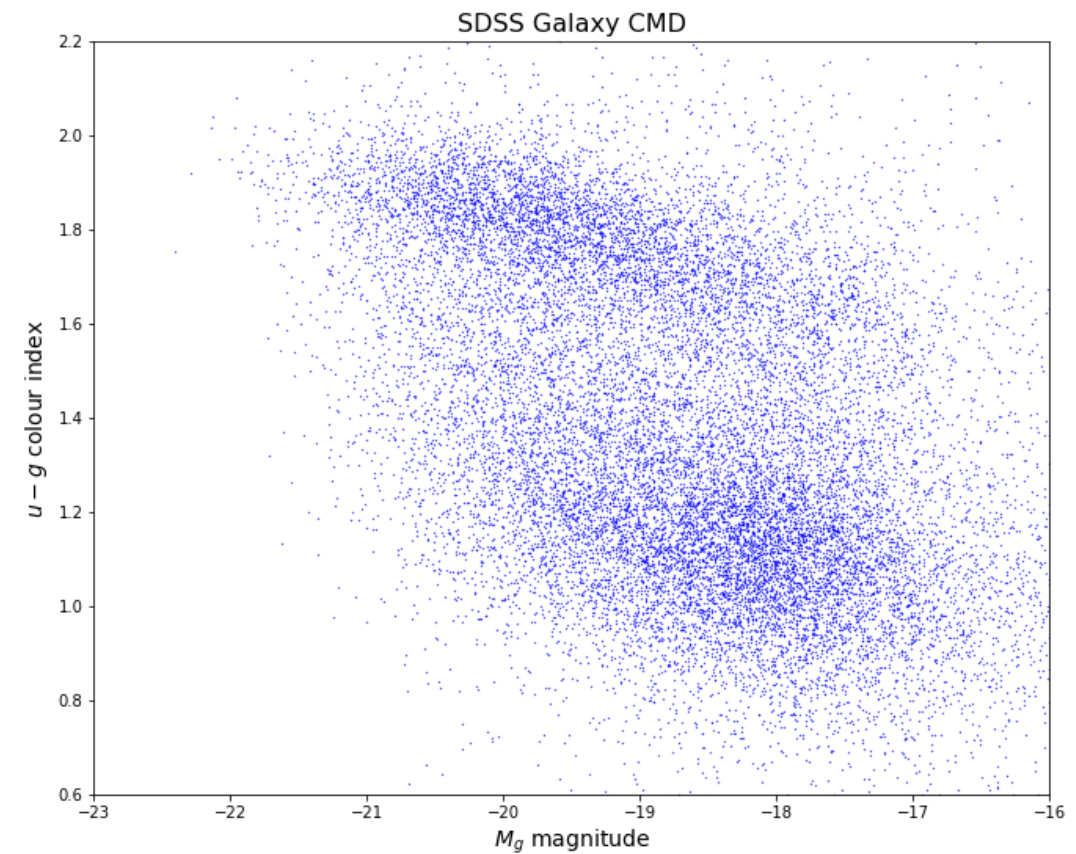
\includegraphics[width=\columnwidth]{images/CMDs/galaxyCMD.PNG}
    \caption[Galaxy CMD]{Galaxy colour-magnitude diagram: the distribution of 20,000 nearby galaxies from the Sloan Digital Sky Survey. The colour index $u-g$ is plotted against $M_g$ magnitude. The distribution exhibits clear bimodality with late-type galaxies occupying a 'blue cloud' in the lower right while early-type galaxies form a 'red sequence' along the upper region of the diagram extending to brighter magnitudes. There is a clearly under-populated band separating the two dense regions, this is the so-called 'green valley'}
    \label{fig:CMD1}
\end{figure}


\begin{figure}
    \centering
    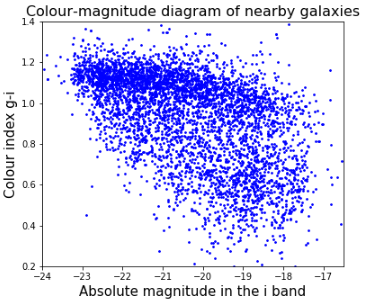
\includegraphics[width=\columnwidth]{images/CMDs/CMD-G_i-i.png}
    \caption{Caption}
    \label{fig:CMD-G_i-i}
\end{figure}

\begin{figure}
    \centering
    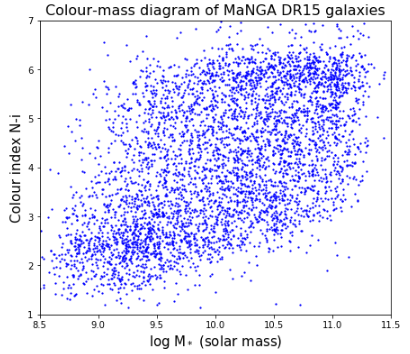
\includegraphics[width=\columnwidth]{images/CMDs/CMD-mass-1.png}
    \caption{Caption}
    \label{fig:CMD-mass-1}
\end{figure}

\subsection{Post starburst Galaxies}

Post-starburst (PSB) galaxies are a class of galaxies where the spectra indicate that star formation has ceased within the past gigayear or so. The is no spectral evidence of young O and B-type stars which will have gone supernova in the dynamical time since the starburst event. PSB spectra are dominated by the strong Balmer absorption lines H$\beta$, H$\gamma$, H$\delta$ indicative of a population of main sequence A- and F-type stars, particularly if a strong  H$\delta$ absorption line width is evident \citep{1997A&A...325.1025P}, while nebular emission lines characteristic of ongoing star formation, for example H$\alpha$ 6564 \AA\ and [OII] 3727\AA\, are weak or absent \citep{2001ApJ...547L..17B,2003PASJ...55..771G,2004MNRAS.355..713B,2005MNRAS.357..937G,2018MNRAS.477.1708P}. The morphology of PSBs is often that of early-type ellipticals and therefore PSBs are often referred to as E+A or K+A galaxies \citep{1983ApJ...270....7D,1996ApJ...466..104Z,2009ARA&A..47..159B}. These spectral observations are characteristic of a brief burst of star formation in the past 0.5 to 1.5 Gyr which has subsequently ceased, or been 'quenched' \citep{1983ApJ...270....7D,1987MNRAS.229..423C,1997A&A...325.1025P}. These spectral features are indicative that PSB galaxies are in transition on an evolutionary track from active star-forming galaxies to passive spheroids \citep{2004MNRAS.355..713B,2012MNRAS.420..672S,2013MNRAS.429.2212M}. Using a sample of a sample of low-redshift (z~0.1) E+A galaxies from the 2dF Galaxy Redshift Survey (2dFGRS) \citet{2004MNRAS.355..713B} find evidence of major mergers such as tidal tails and conclude that major mergers are an important formation mechanism for E+A PSB galaxies. A number of studies have shown that about half of galaxies have experienced recent rapid quenching while an evolutionary track to the red sequence \citep{Martin_2007,10.1111/j.1365-2966.2009.14537.x,2015MNRAS.450..435S}, however see \cite{2017ApJ...845..145W}. Quenching during mergers is also apparent in simulations, see e.g. \cite{2019MNRAS.484.2447D}.

In this study we analyse the kinematic properties of post-starburst galaxies to determine if there is evidence of major mergers in their kinematic signatures, and ask if major mergers could be the primary cause of the cessation of star formation. The objective would be to establish a link between merger activity, the quenching of star formation and morphological transition from blue late-type disc galaxies, through the green valley, to redder passive spheroids.

For this work we utilise a sample of 68 PSBs drawn from the SDSS-IV MaNGA (Mapping Nearby Galaxies at Apache Point Observatory integral field spectroscopic survey  as described in Section \ref{sec:data}.

[TODO: reformulate the following paragraph] See Vivienne's  papers researching PSBs: \citet{2017MNRAS.472.1401A} regarding the relationship of quenching and transition. \citet{2016MNRAS.463..832W} sets out the background work.

\subsection{Structure of the paper}
The content of the paper is organised as follows: A concise review of the literature on galaxy mergers and morphology transitions relevant to the paper is introduced in Section \ref{sec:mergers}. Details of the MaNGA survey and the selection criteria for our PSB sample and control galaxies are provided in Section \ref{sec:data}. Section \ref{sec:kinematics} describes the application of kinematics to the study of galaxy morphology and evolution. The selection criteria for our PSB sample and control galaxies are laid out in Section \ref{sec:data}. Data analysis methods and results are presented in Section \ref{sec:results}. The method of the velocity field analysis method employing the Radon transform method is a significant analysis tool in its own right. This is discussed in some detail in Section \ref{sec:Radon}. Finally, a summary of the research and the conclusions drawn from this work, along with recommendations for further study are presented in Section \ref{sec:discussion}.
